\chapter{Estimadores}
Recordemos que dado un modelo estadístico, nosotros queremos obtener dado los datos, cuál es la ley y más específicamente aún, qué parámetros bajo una ley fueron los cuales generaron la data que se tiene. En este capítulo se introducirá la noción de estimador, función que busca poder aproximar el parámetro mencionado anteriormente.

\section{Estimador}

\begin{definition}
    Sea $g:\Omega\rightarrow \mathbb{R}^n$  tal que $g(\theta) = (g_1(\theta),...,g_n(\theta))$ a valores en $\mathbb{R}$. Nos interesa estimar $g(\theta)$. Para estimar $g(\theta)$ usamos un \textbf{estimador} que es una función $\hat{g}:\mathfrak{X}\rightarrow g(\theta)$ medible. Se dice que $\hat{g(\theta)}$ es la estimación de $g(\theta)$.
    
\end{definition}

Se estudiarán primero los estimadores desde el enfoque frecuentista. Un ejemplo es el siguiente:

\begin{example}[Estimador de la media Gaussiana]
	\label{ex:estimador_media}
	Consideremos $X = (X_1,\ldots,X_n)\sim\cN(\mu,\sigma^2)$. Un estimador de $g(\theta) = g(\mu,\sigma) = \mu$ es el estadístico 
	\begin{equation}
	\nonumber
		\gh(X) = \frac{1}{n}\sum_{i=1}^nX_i
	\end{equation} 
\end{example}

\section{Estimadores insesgados} 
Una clase muy importante de estimadores son los estimadores insesgados. 

\begin{definition}[Estimador insesgado]
	\label{def:estimador_insesgado}
	Sea $\ghx$ un estimador de $g(\theta)$. Este estimador es insesgado si 
	\begin{equation}
	\nonumber
		\E{\ghx} = g(\theta)
	\end{equation}
	y el sesgo de $\gh$ se define como 
	\begin{equation}
	\nonumber
		b_\gh(\theta) = \E{\ghx} - g(\theta)
	\end{equation}
	Se dice también que un estimador es \textbf{asintoticamente insesgado} si es que:
	\[\lim_n\E{\gh (x_1,...,x_n)} = g(\theta)\]
\end{definition}



Los estimadores insesgados juegan un rol importante en el estudio y aplicación de la estadística, sin embargo, uno no siempre debe poner exclusiva atención a ellos (dado que no siempre son los 'mejores', este concepto se estudiará más adelante). Los siguientes ejemplos ilustran el rol del estimador insesgado en dos familias paramétricas distintas. 

\begin{example}[Estimador insesgado de la media Gaussiana]
	\label{ex:estimador_in_media}
	El estimador de $g(\theta) =  \mu$ descrito en el Ejemplo \ref{ex:estimador_media} es insesgado, en efecto: 
	\begin{equation}
	\nonumber
		\E{\ghx} = \E{\frac{1}{n}\sum_{i=1}^nX_i}	= \frac{1}{n}\sum_{i=1}^n\E{X_i}		= \frac{1}{n}\sum_{i=1}^n\mu = \mu	
	\end{equation}
\end{example}


\begin{example}[Estimador de la taza de la distribución exponencial\footnote{Schervish}]
	\label{ex:estimador_exponancial}
	Consideremos $X\sim Exp(\theta)$, donde $Exp(x|\theta) = \theta\exp(-\theta x)$, y asumamos que existe un estimador insesgado $\ghX$ de $g(\theta) = \theta$, entonces, 
	\begin{equation}
	\nonumber
		\E{\ghX} = \int_0^\infty \ghx\theta\exp(-\theta x)\d x = \theta, \forall \theta,
	\end{equation}
	lo cual es equivalente a decir que $\int_0^\infty \ghx\exp(-\theta x)\d x = 1, \forall \theta$ o bien que (al derivar ambos lados de esta expresión c.r.a. $\theta$)  $\int_0^\infty x\ghx\exp(-\theta x)\d x = 0, \forall \theta$.\\

	Esta última expresión es equivalente a que $\E{X\ghX} = 0$, lo que a su vez y considerando que $X$ es un estadístico suficiente y completo, implica que necesariamente la función $X\ghX=0$ c.s. $\forall \theta$, y también que $\ghX=0$ c.s. $\forall \theta$. Como esto contradice el hecho de que $\ghX$ es insesgado, no es posible construir estimadores insesgados para $\theta$ en la distribución exponencial.
\end{example}


Veamos ahora un ejemplo de un estimador sesgado de la varianza y cómo se puede construir un estimador insesgado. 

\begin{example}
Consideremos una familia paramétrica $\familiaparametrica$ y denotemos por $\mu$ y $\sigma^2$ su media y su varianza respectivamente. Usando las observaciones $x_1,x_2,\ldots,x_n$, calculemos la varianza del estimador de la media, dado por $\xb = \frac{1}{n}\sum_{i=1}^n x_i$ mediante
\begin{equation}
	\label{eq:varianza_media_muestral}
 	\Vt{\xb} = \Vt{\frac{1}{n}	\sum_{i=1}^n x_i}  \underbrace{=}_{\text{i.i.d.}}  \frac{1}{n^2}	\sum_{i=1}^n\Vt{ x_i} =\frac{\sigma^2}{n}
 \end{equation} 
 es decir, el estimador de la media usando $n$ muestras, tiene una varianza $\sigma^2/n$.

 Consideremos ahora el siguiente estimador para la varianza: 
\begin{equation}
	\label{eq:est_varianza_sesgado}
	S_2 = \frac{1}{n}\sum_{i=1}^n (x_i-\xb)^2
\end{equation}
y notemos que la esperanza de dicho estimador es
\begin{align}
	\label{eq:sesgo_varianza}
	\Et{S_2 } &= \Et{\frac{1}{n}\sum_{i=1}^n (x_i-\mu+\mu-\xb)^2}\nonumber\\
				&= \Et{ \frac{1}{n}\sum_{i=1}^n(x_i-\mu)^2 + 2\frac{1}{n}\sum_{i=1}^n(x_i-\mu)(\mu-\xb) + \frac{1}{n}\sum_{i=1}^n(\mu-\xb)^2}\nonumber\\
				&= \Et{ \frac{1}{n}\sum_{i=1}^n(x_i-\mu)^2 - 2(\mu-\xb)^2 + (\mu-\xb)^2}\nonumber\\
				&= \Et{ \frac{1}{n}\sum_{i=1}^n(x_i-\mu)^2 - (\mu-\xb)^2}\nonumber\\
				&= \Vt{x_i} - \Vt{\xb}\quad\text{ver ecuación \eqref{eq:varianza_media_muestral}}\nonumber\\
				&= 	\sigma^2 + \sigma^2/n = \left(\frac{n+1}{n}\right)\sigma^2
\end{align}
Esto quiere decir que el sesgo del estimador en la ecuación \eqref{eq:est_varianza_sesgado} es asintóticamente insesgado, es decir, que su sesgo tiende a cero cuando el número de muestas $n$ tiende a infinito. Sin embargo, notemos que podemos corregir el estimador de la varianza multiplicando el estimador original, $S_2$ en la ecuación \eqref{eq:est_varianza_sesgado} por $n/(n+1)$, con lo que el estimador corregido denotado por 
\begin{equation}
	\label{eq:est_varianza_insesgado}
	S'_2 = \frac{n}{n+1}S_2 =  \frac{1}{n+1}\sum_{i=1}^n (x_i-\xb)^2
\end{equation}
cumple con
\begin{equation}
	\Et{S'_2 } =  \left(\frac{n}{n+1}\right)\Et{S_2} \underbrace{=}_{\text{ec.}\eqref{eq:sesgo_varianza}} \left(\frac{n}{n+1}\right) \left(\frac{n+1}{n}\right)\sigma^2 = \sigma^2
\end{equation}
es decir, el estimador $S'_2$ en la ecuación \eqref{eq:est_varianza_insesgado} es insesgado.
\end{example}

\section{Funciones de perdida}

\begin{definition}
Una función de pérdida (también llamadas función de costos) es una función a valores reales de dos variables, $L(\theta,a) $, donde $\theta \in \Omega$ y $a \in \R$. 
\end{definition}

La función de pérdida más ocupada es el \textbf{error cuadrático}. Esta función está dada por: 
$$
L(\theta,a) = (\theta-a)^{2}
$$

Luego, como el estimador es una VA, también lo es la función de pérdida, por lo que podemos calcular la esperanza de la función de pérdida, lo cual conocemos como \textit{riesgo}. El riesgo asociado a la pérdida cuadrática en la ecuación anterior está dado por: 
\begin{alignat}{3}
 	R(\theta, \hat{g})  &= \E{(\theta - \phi)^2}\nonumber\\
 						& = \E{\left(\theta - \bar{\phi}+ \bar{\phi} -\phi\right)^2}; \quad \text{denotando }\bar{\phi} = \E{ \phi}\nonumber\\
 						& = \E{(\theta - \bar{\phi})^2+2(\theta - \bar{\phi})\cancel{(\bar{\phi} -\phi)} +  (\bar{\phi} -\phi)^2}\nonumber\\
 						& = \underbrace{(\theta - \bar{\phi})^2}_{=b_{\phi}^2\ (\text{sesgo}^2)} +  \underbrace{\E{(\bar{\phi} -\phi)^2}}_{=V_{\phi}\ \text{(varianza)}}.\label{eq:riesgo_cuad}
 \end{alignat} 

\section{Teorema de Rao-Blackwell}
Para tener una notación más limpia, desde ahora nos referiremos a estimadores $\phi=\gh$ de $\theta$ en general para evitar la expresión más engorrosa estimador $\gh(X)$ de $g(\theta)$.



Como ya vimos, es natural evaluar la bondad de distintos estimadores (sesgados o insesgados) mediante una función de \textit{pérdida} o \textit{costo} que compara el valor reportado por el estimador y el valor real del parámetro. Es decir, usamos la función de pérdida como una métrica para comparar estimadores.\\

El siguiente teorema establece que la información reportada por un estadístico suficiente (Definición \ref{def:estadístico_suficiente}), puede solo mejorar un estimador. 

\begin{theorem}[Teorema de Rao-Blackwell]
	\label{teo:rao-blackwell}
	Sea $\phi = \phi(X)$ un estimador de $\theta$ tal que $\Et{\phi}<\infty, \forall \theta$. Asumamos que existe $T$ estadístico suficiente para $\theta$ y sea $\phi^\star = \Et{\phi|T}$. Entonces, 
	\begin{equation}
		\Et{(\phi^\star-\theta)^2} \leq \Et{(\phi-\theta)^2}, \forall\theta,
	\end{equation}
	donde la desigualdad es estricta salvo en el caso donde $\phi$ es función de $T$.
\end{theorem}

En otras palabras, el Teo. de Rao-Blackwell establece que un estimador puede ser \textit{mejorado} si es reemplazado por su esperanza condicional dado un estadístico suficiente. El proceso de mejorar un estimador poco eficiente de esta forma es conocido como \textit{Rao-Blackwellización} y veremos un ejemplo a continuación.


\begin{example}
Consideremos $X = (X_1,\ldots,X_n)\sim \poi{\theta}$ y estimemos el parámetro $\theta$. Para esto, consideremos el estimador básico $\phi = X_1$ y \textit{Rao-Blackwellicémoslo} usando el estimador suficiente $T=\sum_{i=1}^nX_i$, es decir, 
\begin{equation}
	\phi^* = \Et{X_1\middle|\sum_i X_i=t}.
\end{equation}
Para calcular esta esperanza condicional, observemos primero que  
\begin{equation}
	\sum_{j=1}^n\Et{X_j\middle|\sum_{i=1}^n X_i=t} = \Et{\sum_{j=1}^nX_j\middle|\sum_{i=1}^n X_i=t} = t
\end{equation}
y que como $X_1,\ldots,X_n$ son iid, entonces todos los términos dentro de la suma del lado izquierdo de la ecuación anterior son iguales. Consecuentemente, recuperamos el estimador
\begin{equation}
 	\phi^* = \frac{t}{n} = \frac{1}{n}\sum_{i=1}^nX_i
 \end{equation} 
\end{example}

Para demostrar el Teorema \ref{teo:rao-blackwell} consideremos dos variable aleatorias $X\in\cX$, $Y\in\cY$, y recordemos dos propiedades básicas. En primer lugar la ley de esperanzas totales, la cual establece que 
\begin{alignat}{3}
	\mathbb{E}_Y{\mathbb{E}_{X|Y}{(X|Y)}} &= \int_\cY\int_\cX x \d P(x|y) \d P(y) \quad\quad&&\text{def. esperanza}\nonumber\\
				&=  \int_\cX x \int_\cY \d P(x|y) \d P(y) &&\text{linealidad}\nonumber\\
				&=  \int_\cX x \int_\cY \d P(x,y) &&\text{def. esperanza condicional}\nonumber\\
				&=  \int_\cX x \d P(x) = \mathbb{E}_X(X) &&\text{def. esperanza} \label{eq:total_expectation}
\end{alignat}
y la desigualdad de Jensen, la cual para el caso particular del costo cuadrático, puede verificarse que
\begin{equation}
	0 \leq \V{X} =  \E{X^2}-\E{X}^2 \Rightarrow \E{X^2} \geq \E{X}^2. \label{eq:jensen_var}
\end{equation}
La desigualdad de Jensen es geométricamente intuitiva, como se observa en la figura \ref{fig:intuicion_jensen}. Al calcular la imágen de $\mathbb{E}(x)$ bajo una función convexa, podemos encontrar una recta tangente a ese punto $L(X)=aX+b$. Tendremos que $\mathbb{E}(\varphi(X')) \geq \mathbb{E}(L(X'))=\mathbb{E}[aX'+b]=a\mathbb{E}[X`]+b=L(\mathbb{E}(X'))$ para otro punto $X'$. Tomando $X'=X$, $\mathbb{E}(\varphi(X)) \geq \varphi(\mathbb{E}(X))$.
\begin{figure}[h]
    \centering
    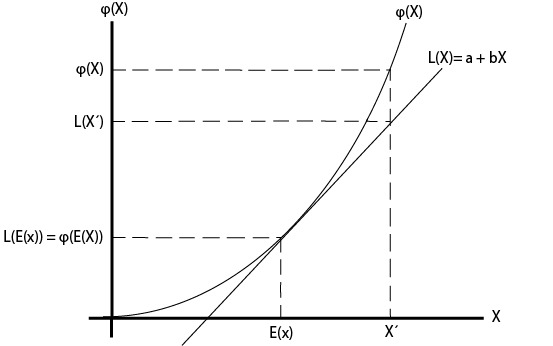
\includegraphics[scale=0.5]{img/Intuicion_Jensen.jpeg}
    \caption{Intuición geométrica de la desigualdad de Jensen }
    \label{fig:intuicion_jensen}
\end{figure}

Volviendo a lo anterior, utilizando las expresiones en \eqref{eq:total_expectation} y \eqref{eq:jensen_var}, podemos demostrar el teorema anterior.

 \begin{proof}[Demostración de Teorema \ref{teo:rao-blackwell}]
 	La varianza del estimador $\phi^\star$ está dada por 
 	\begin{alignat*}{2}
 		\Et{(\phi^\star-\theta)^2} &= \Et{(\Et{\phi|T}-\theta)^2} \quad\quad\quad &&\text{def.}\\
 								&= \Et{(\Et{\phi-\theta|T})^2}&& \text{linealidad}\\
 								&\leq \Et{\Et{(\phi-\theta)^2|T}}&& \text{Jensen}\\
 								&= \Et{(\phi-\theta)^2} &&\text{ley esperanzas totales}
 	\end{alignat*}
Donde las esperanzas exteriores son con respecto a $T$ y las interiores con respecto a $X$ (o equivalentemente a $\phi$).  Observemos además que la desigualdad anterior viene de la expresión en la ecuación \eqref{eq:jensen_var}, por lo que la igualdad es obtenida si $\V{\phi-\theta|T} = 0$, es decir, la VA $\phi-\theta$ tiene que ser constante para cada valor de $T$, es decir, $\phi$ es función de $T$. Intuitivamente podemos entender esto como que si el estadístico ya fue considerado en el estimador, entonces conocer el valor del estadístico no reporta información adicional. 
 \end{proof}

\begin{remark}
	Notemos que si el estimador $\phi$ es insesgado, su \textit{Rao-Blackwellización} $\phi^*$ también lo es, en efecto
	\begin{equation}
		\Et{\phi^*} = \Et{\Et{\phi|T}} = \Et{\phi} = \theta,
	\end{equation}
	donde la segunda igualdad está dada por la ley de esperanzas totales y la tercera por el supuesto de que $\phi$ es insesgado.
\end{remark}

\section{Varianza uniformemente mínima}

En base al riesgo cuadrático definido en la ecuación \eqref{eq:riesgo_cuad}, podemos ver que si un estimador es insesgado (Definición \ref{def:estimador_insesgado}), su riesgo cuadrático es únicamente su varianza. Esto motiva la siguiente definición de optimalidad para estimadores insesgados. 

 \begin{definition}[Estimador insesgado de varianza uniformemente mínima]
  	El estimador $\phi$ de $\theta$ es un estimador insesgado de varianza uniformemente mínima (EIVUM) si es insesgado y si $\forall \phi':\cX\rightarrow \Theta$ estimador insesgado se tiene
  	\begin{equation}
  		\Vt{\phi}\leq\Vt{\phi'}, \forall \theta\in\Theta.
  	\end{equation}
  \end{definition} 

\begin{example}
	Consideremos $x=(x_1,\ldots,x_n)\sim\ber{\theta}$ y los siguientes estimadores de $\theta$
	\begin{itemize}
		\item $\phi_1(x) = x_1$
		\item $\phi_2(x) = \frac{1}{2}(x_1+x_2)$
		\item $\phi_3(x) = \frac{1}{n}\sum_{i=1}^n x_i$
	\end{itemize}
	Observemos que todos estos estimadores son insesgados, pues como $\forall i, \Et{x_i} = \theta$, entonces 
	\begin{equation}
		\Et{\phi_1(x)} = \Et{\phi_2(x)} = \Et{\phi_3(x)} = \theta
	\end{equation}
	Veamos ahora que la varianza de $\phi_3(x)$ está dada por
	\begin{equation}
		\Vt{\phi_3(x)} = \Vt{\frac{1}{n}\sum_{i=1}^n x_i} = \frac{1}{n^2}\sum_{i=1}^n \Vt{x_i} = \frac{\theta(1-\theta)}{n}
	\end{equation}
	pues $\Vt{x_i} = \Et{(\theta - x_i)} = \Et{x_i^2} - \theta^2 = (0^2 \cdot (1-\theta) + 1^2 \cdot \theta) - \theta^2 = \theta(1-\theta)$. Consecuentemente, la varianza de los estimadores considerados decae como la inversa del número de muestras.
\end{example}

Con las definiciones anteriores, podemos mencionar el siguiente teorema, el cual conecta la noción de estadístico completo con la de EIVUM. 

\begin{theorem}[Teorema de Lehmann-Scheffé]
	Sea $X$ una VA con distribución paramétrica $\familiaparametrica$ y $T$ un estadístico suficiente y completo para $\theta$. Si el estimador $\phi = \phi(T)$ de $\theta$ es insesgado, entonces $\phi$ es el único EIVUM. 
 \end{theorem} 

 \begin{proof}
 	Veamos en primer lugar que es posible construir un estimador en función del estadístico $\phi(T)$ que tiene menor o igual varianza que un estimador arbitrario $\phi'(X)$. En efecto, el Teorema de Rao-Blackwell estable ce que el estimador 
 	\begin{equation}
 		\phi(T) = \Et{\phi'(X)|T},
 	\end{equation}
 	tiene efectivamente menos varianza que $\phi'(X)$.\\

 	Ahora veamos que solo existe un único estimador insesgado que es función de $T$, en efecto, si existiesen dos estimadores insesgados de $\theta$, $\phi_1(T),\phi_2(T)$, entonces, $\Et{\phi_1(T)-\phi_1(T)}=0$ y como $T$ es completo, entonces, $\phi_1(T) = \phi_2(T)$ c.s.-$P_\theta$.\\

 	Hemos probado que (i) para un estimador arbitrario, se puede construir un estimador que es función de $T$ el cual tiene menor o igual varianza que el estimador original y, (ii) el estimador insesgado $\phi(T)$ es único. Consecuentemente, $\phi(T)$ es el único EIVUM.
 \end{proof}

El Teorema de Lehmann-Scheffé da una receta para encontrar el EIVUM: simplemente es necesario encontrar un estadístico completo y construir un estimador insesgado en base a éste, esto garantiza que el estimador construido es el \textbf{único} EIVUM.
\begin{example}[EIVUM para Bernoulli]
	Recordemos que en el Ejemplo \ref{eq:est_completo_bernoulli} vimos que el estadístico $T=\sum_{i=1}^nX_i$ es completo para $X\sim\ber{\theta}$. Como el estimador de $\theta$ dado por $\phi(T) = T/n$ es insesgado, 
\begin{equation}
	\Et{\phi(T)} = \Et{T/n} = \sum_{i=1}^n \Et{X_i} /n = \theta,
\end{equation}
entonces $\phi(T) = T/n$ es el EIVUM para $\theta$ en $\ber{\theta}$.	
\end{example}
